\chapter{Evaluation \& Testing}\label{ch:Evaluation}
\section{Results}
\subsection{Random Forest: algorithm baseline performance}
As explained in Chapter 4, the first experiment to be conducted was to feed the datasets through  a Random Forest algorithm and record the performance metrics for each dataset as a baseline to compare the results of the following experiments to. Full script for this experiment can be found in Experiment1.R.

The confusion matrix was obtained from the RandomForestModelling.R script for each dataset is shown in appendix D1-D10 and was used to further interpret the data shown in table 5.1.\newline
Table 5.1 shows the results obtained for each dataset. There are three occasions where the performance metrics were not calculated:
\begin{itemize}
    \item The precision value for the Fertility dataset
    \item The F1 value for the Fertility dataset
    \item The F1 value for the modified Heart Attack dataset
\end{itemize}

\begin{table}[!htbp]
\centering
\begin{tabular}{lrrrr}
  \hline
  \rowcolor{LightCyan}
Dataset & Accuracy & Sensitivity & Precision & F1Score \\ 
  \hline
AuSDf & 1.00 & 1.00 & 1.00 & 1.00 \\ 
  BCDf & 0.92 & 0.86 & 0.94 & 0.89 \\ 
  CCDf & 1.00 & 0.90 & 1.00 & 0.95 \\ 
  DiabetesDf & 0.74 & 0.56 & 0.72 & 0.63 \\ 
  FertDf & 0.93 & 0.00 & nd & nd \\ 
  HAPDf & 0.91 & 0.83 & 0.89 & 0.86 \\ 
  LBPDf & 0.82 & 0.90 & 0.84 & 0.87 \\ 
  LiverDf & 0.72 & 0.35 & 0.58 & 0.44 \\ 
  subHAPDf & 0.95 & 0.00 & 0.00 & nd \\ 
  subLBPDf & 0.91 & 0.50 & 1.00 & 0.67 \\ 
   \hline
\end{tabular}
\caption{Performance metrics obtained for Random Forest applied to the chosen datasets}
\end{table}

The data from the confusion matrix output for the Fertility test (Appendix D.5)
show that there were no accurate prediction for the positive class and no inaccurate prediction for the positive class which means the the Precision or Positive predictive value could not be calculated (no division by 0) for this dataset. A lack of Precision value means that the F1 score cannot be calculated as it is obtained by calculated the harmonic mean of Precision and Sensitivity.\newline
This result is partly due to the size of the dataset (only 100 observations and as such there are only 29 observations in the test set). This means that the model will very accurately predict people not suffering infertility but struggles to identify people suffering from infertility.\newline
There is no value for the F1 score of the modified Heart Attack dataset as both the Precision and Sensitivity values are equal to 0 and as such the harmonic mean cannot be calculated (no division by 0).

Table 5.1 also shows that only considering overall accuracy when estimating the performance of an algorithm is misleading. Random Forest returns good to very good accuracy for most of these datasets (accuracy ranges from 0.72 to 1), however, excluding the Autism dataset, the Sensitivity, Precision and F1 score obtained can indicate that although the accuracy is good there is a high chance of the algorithm returning a high number of false positives or missing out positives. \newline
Since in all cases except the Low Back Pain dataset, there is a majority of cases for the negative class, this is expected and experimenting with under-sampling and over-sampling of the data may lead to improvement of some of the metrics.


\subsection{Under-sampling of the majority class}
\subsubsection{Retaining 75\% of the majority class}
The first of the under-sampling experiments was to retain 75\% of the majority class. Table 5.2 shows the performance metrics obtained after this operation. Full scripts for this experiments can be found in the Experiment2.R file.
Statistical Analysis on the observed differences for these values is carried out on in the next section 5.2.
The output for the confusion matrix for this experiment are found in Appendix D11-D20.

\begin{table}[ht]
\centering
\begin{tabular}{lrrrr}
  \hline
  \rowcolor{LightCyan}
Dataset & Accuracy & Sensitivity & Precision & F1Score \\ 
  \hline
AuSDf & 1.00 & 1.00 & 1.00 & 1.00 \\ 
  BCDf & 0.88 & 0.91 & 0.81 & 0.86 \\ 
  CCDf & 0.99 & 0.90 & 1.00 & 0.95 \\ 
  DiabetesDf & 0.76 & 0.69 & 0.75 & 0.72 \\ 
  FertDf & 0.91 & 0.33 & 1.00 & 0.50 \\ 
  HAPDf & 0.84 & 0.79 & 0.84 & 0.82 \\ 
  LBPDf & 0.81 & 0.89 & 0.87 & 0.88 \\ 
  LiverDf & 0.62 & 0.47 & 0.50 & 0.49 \\ 
  subHAPDf & 0.98 & 0.00 &  &  \\ 
  subLBPDf & 0.96 & 0.80 & 1.00 & 0.89 \\ 
   \hline
\end{tabular}
\caption{Performance metrics obtained for Random Forest when applied to the chosen datasets after under-sampling the data (75\% majority class retained)}
\end{table}

When 25\% of the majority class was discarded, there was no observable effect on the performance of the algorithm for the Autism dataset.
\begin{itemize}
    \item Breast Cancer dataset: overall accuracy, precision and F1 scored showed a decrease while sensitivity showed an increase.
    \item Cervical Cancer dataset: overall accuracy showed a decrease while other metrics remained unchanged.
    \item Diabetes dataset: all metrics showed an increase.
    \item Fertility dataset: the overall accuracy showed a decrease while sensitivity shows an increase and the precision value can now be calculated (as well as as F1 score).
    \item Heart Attack dataset: all metrics showed a decrease
    \item Low Back Pain dataset: overall accuracy and sensitivity showed a decrease while precision and F1 score showed an increase.
    \item Liver dataset: overall accuracy and precision showed a decrease while the sensitivity and F1 score showed an increase.
    \item Modified Heart Attack dataset: overall accuracy increases but the sensitivity remains at 0 and the precision and F1 score cannot be calculated.
    \item Modified Low Back Pain: the overall accuracy, sensitivity and F1 score showed an increase while precision remained unchanged.
\end{itemize}

Excluding Diabetes, modified Heart Attack and modified Low Back Pain datasets, under-sampling in this case results in a reduced accuracy, and for most cases sensitivity increases. 


\subsubsection{Retaining 60\% of the majority class}
The second of the under-sampling experiments was to retain 60\% of the majority class. Table 5.3 shows the performance metrics obtained after this operation. Full scripts for this experiments can be found in the Experiment2.R file.
Statistical Analysis on the observed differences for these values is carried out on in the next section 5.2.
The output for the confusion matrix for this experiment are found in Appendix D21-30.

\begin{table}[ht]
\centering
\begin{tabular}{lrrrr}
  \hline
  \rowcolor{LightCyan}
Dataset & Accuracy & Sensitivity & Precision & F1Score \\ 
  \hline
AuSDf & 1.00 & 1.00 & 1.00 & 1.00 \\ 
  BCDf & 0.98 & 0.95 & 1.00 & 0.97 \\ 
  CCDf & 0.99 & 0.91 & 0.91 & 0.91 \\ 
  DiabetesDf & 0.76 & 0.79 & 0.73 & 0.76 \\ 
  FertDf & 0.59 & 0.00 & 0.00 &  \\ 
  HAPDf & 0.88 & 0.82 & 0.88 & 0.85 \\ 
  LBPDf & 0.82 & 0.95 & 0.85 & 0.90 \\ 
  LiverDf & 0.59 & 0.62 & 0.48 & 0.55 \\ 
  subHAPDf & 0.89 & 0.20 & 1.00 & 0.33 \\ 
  subLBPDf & 0.85 & 0.40 & 1.00 & 0.57 \\ 
   \hline
\end{tabular}
\caption{Performance metrics obtained for Random Forest when applied to the chosen datasets after under-sampling the data (60\% majority class retained)}
\end{table}

Retaining 60\% of the majority class does not appear to affect the performance of the algorithm and the Autism dataset, where all metrics have achieved maximum value.
\begin{itemize}
    \item Breast Cancer dataset: all metrics show an increase compared to those values obtained from Random Forest on the full dataset.
    \item Cervical Cancer dataset:sensitivity is increased in this case, while the other metrics all show a decrease.
    \item Diabetes dataset:all metrics show an increase compared to those values obtained from Random Forest on the full dataset.
    \item Fertility dataset: the overall accuracy shows an increase while the other metrics remain unchanged.
    \item Heart Attack dataset: all metrics show a decrease in this situation
    \item Low Back Pain dataset: the overall accuracy is unchanged while sensitivity, precision and F1 score all show an increase.
    \item Liver dataset:Sensitivity and F1 score show an increase while accuracy and precision show a decrease
    \item Modified Heart Attack dataset: the overall accuracy is decreased but both sensitivity and precision have increased and F1 score can now be calculated as both values are $>$0.
    \item Modified Low Back Pain dataset: Overall accuracy and sensitivity show a decrease while precision remains the same and the F1 score increases.
\end{itemize}

Discarding 40\% of the majority class generally leads to a decrease in overall accuracy (apart from the Breast Cancer dataset) and an increase in sensitivity (apart from the Heart Attack dataset), the effect on precision is variable and effect on the F1 score values depends on the extent of the variation observed on sensitivity and precision.

\subsubsection{Retaining 40\% of the majority class}
The first of the under-sampling experiments was to retain only 40\% of the majority class. Table 5.4 shows the performance metrics obtained after this operation. Full scripts for this experiments can be found in the Experiment2.R file.
The output for the confusion matrix for this experiment are found in Appendix D31-40.

\begin{table}[ht]
\centering
\begin{tabular}{lrrrr}
  \hline
  \rowcolor{LightCyan}
Dataset & Accuracy & Sensitivity & Precision & F1Score \\ 
  \hline
AuSDf & 1.00 & 1.00 & 1.00 & 1.00 \\ 
  BCDf & 0.95 & 0.95 & 0.97 & 0.96 \\ 
  CCDf & 0.97 & 1.00 & 0.81 & 0.90 \\ 
  DiabetesDf & 0.69 & 0.83 & 0.70 & 0.76 \\ 
  FertDf & 0.82 & 0.00 &  &  \\ 
  HAPDf & 0.79 & 0.89 & 0.76 & 0.82 \\ 
  LBPDf & 0.82 & 1.00 & 0.82 & 0.90 \\ 
  LiverDf & 0.65 & 0.74 & 0.61 & 0.67 \\ 
  subHAPDf & 0.92 & 0.00 & 0.00 &  \\ 
  subLBPDf & 1.00 & 1.00 & 1.00 & 1.00 \\ 
   \hline
\end{tabular}
\caption{Performance metrics obtained for Random Forest when applied to the chosen datasets after under-sampling the data (40\% majority class retained)}
\end{table}

Interestingly the performance of Random Forest on the Autism dataset after under-sampling is not affected at all. Although 60\%of the majority class has been discarded, all the metrics have achieved maximum value.
Statistical Analysis on the observed differences for these values is carried out on in the next section 5.2.
\begin{itemize}
    \item Breast Cancer dataset: there is an increase in all metrics compared to those obtained with the full dataset 
    \item Cervical Cancer dataset: there is a decrease in overall accuracy, precision and F1 score, however there is an increase in sensitivity.
    \item Diabetes dataset: there is a decrease in overall accuracy and precision but an increase in sensitivity and F1 score.
    \item Fertility dataset: there is a decrease in overall accuracy and the other metrics remain the same.
    \item Heart Attack dataset: there is a decrease in accuracy, precision and F1 score whereas sensitivity has increased.
    \item Low Back Pain dataset: there is a decrease in accuracy and precision but the F1 score and sensitivity have both increased.
    \item Liver Dataset: all metrics except overall accuracy have increased.
    \item Modified Heart Attack dataset: there is a decrease in overall accuracy and all other values remain unchanged
    \item Modified Low Back Pain: all metrics show an increase apart from precision which remains unchanged
\end{itemize}

The variations between the performance metrics obtained for each of the under-sampling conditions were calculated compared to the established baseline in experiment 1.\newline
The variations for Accuracy, Sensitivity, Precision and Accuracy are shown in the Appendix tables D1-D4.
These values were used to create graphs to represent the variations for each metrics in the different conditions and for the different datasets.\newline


\begin{figure}[!htbp]
    \centering
    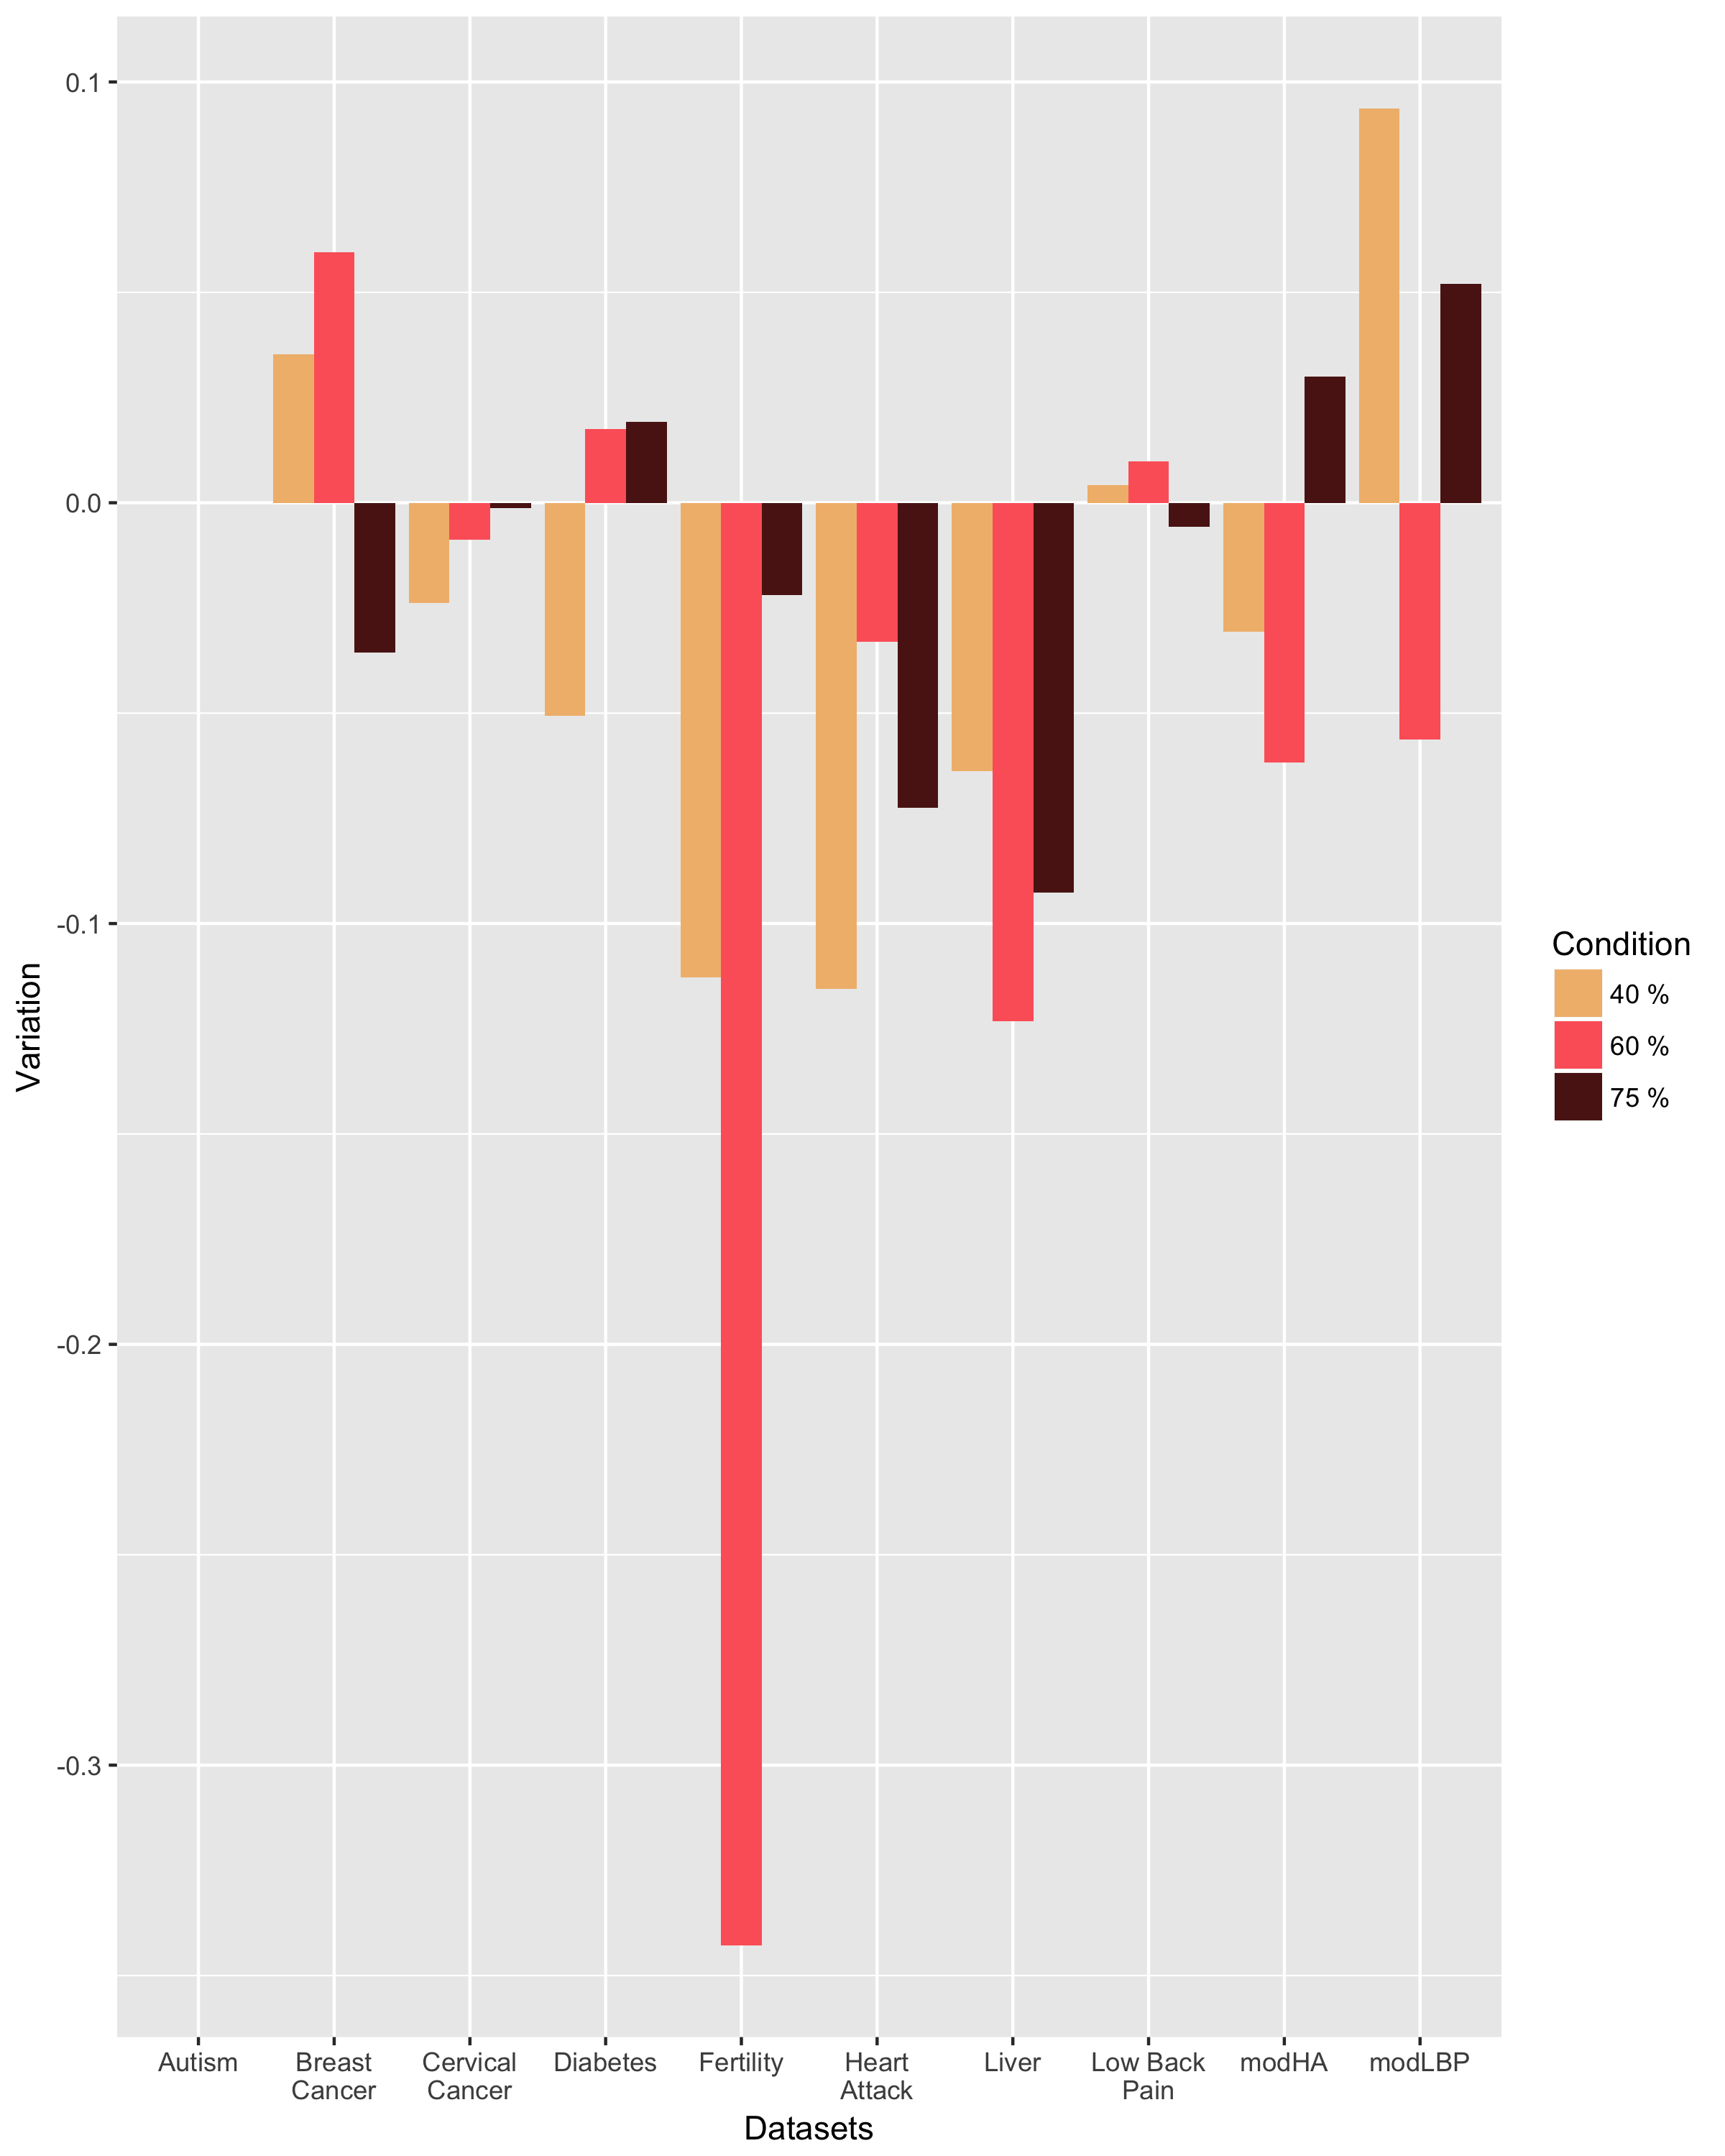
\includegraphics[width=0.9\textwidth]{ThesisTemplate/usingLatex/chapter5Images/AccuVariationUnderBySets.png}
    \caption{Variation of the accuracy value for the three under-sampling conditions compared to the baseline established in Experiment 1 for all studied datasets.}
    \label{fig:my_label}
\end{figure}

Figure 5.1 shows the variations in accuracy observed when 75\%, 60\% and 40\% of the majority class was retained.
Overall the effect is that of a decrease in accuracy when under-sampling of the  majority class is applied, though the effect is slight (less than 0.15 variation for most datasets, except for the Diabetes dataset where the accuracy is greatly affected when under-sampling occurs).\newline



\begin{figure}[!htbp]
    \centering
    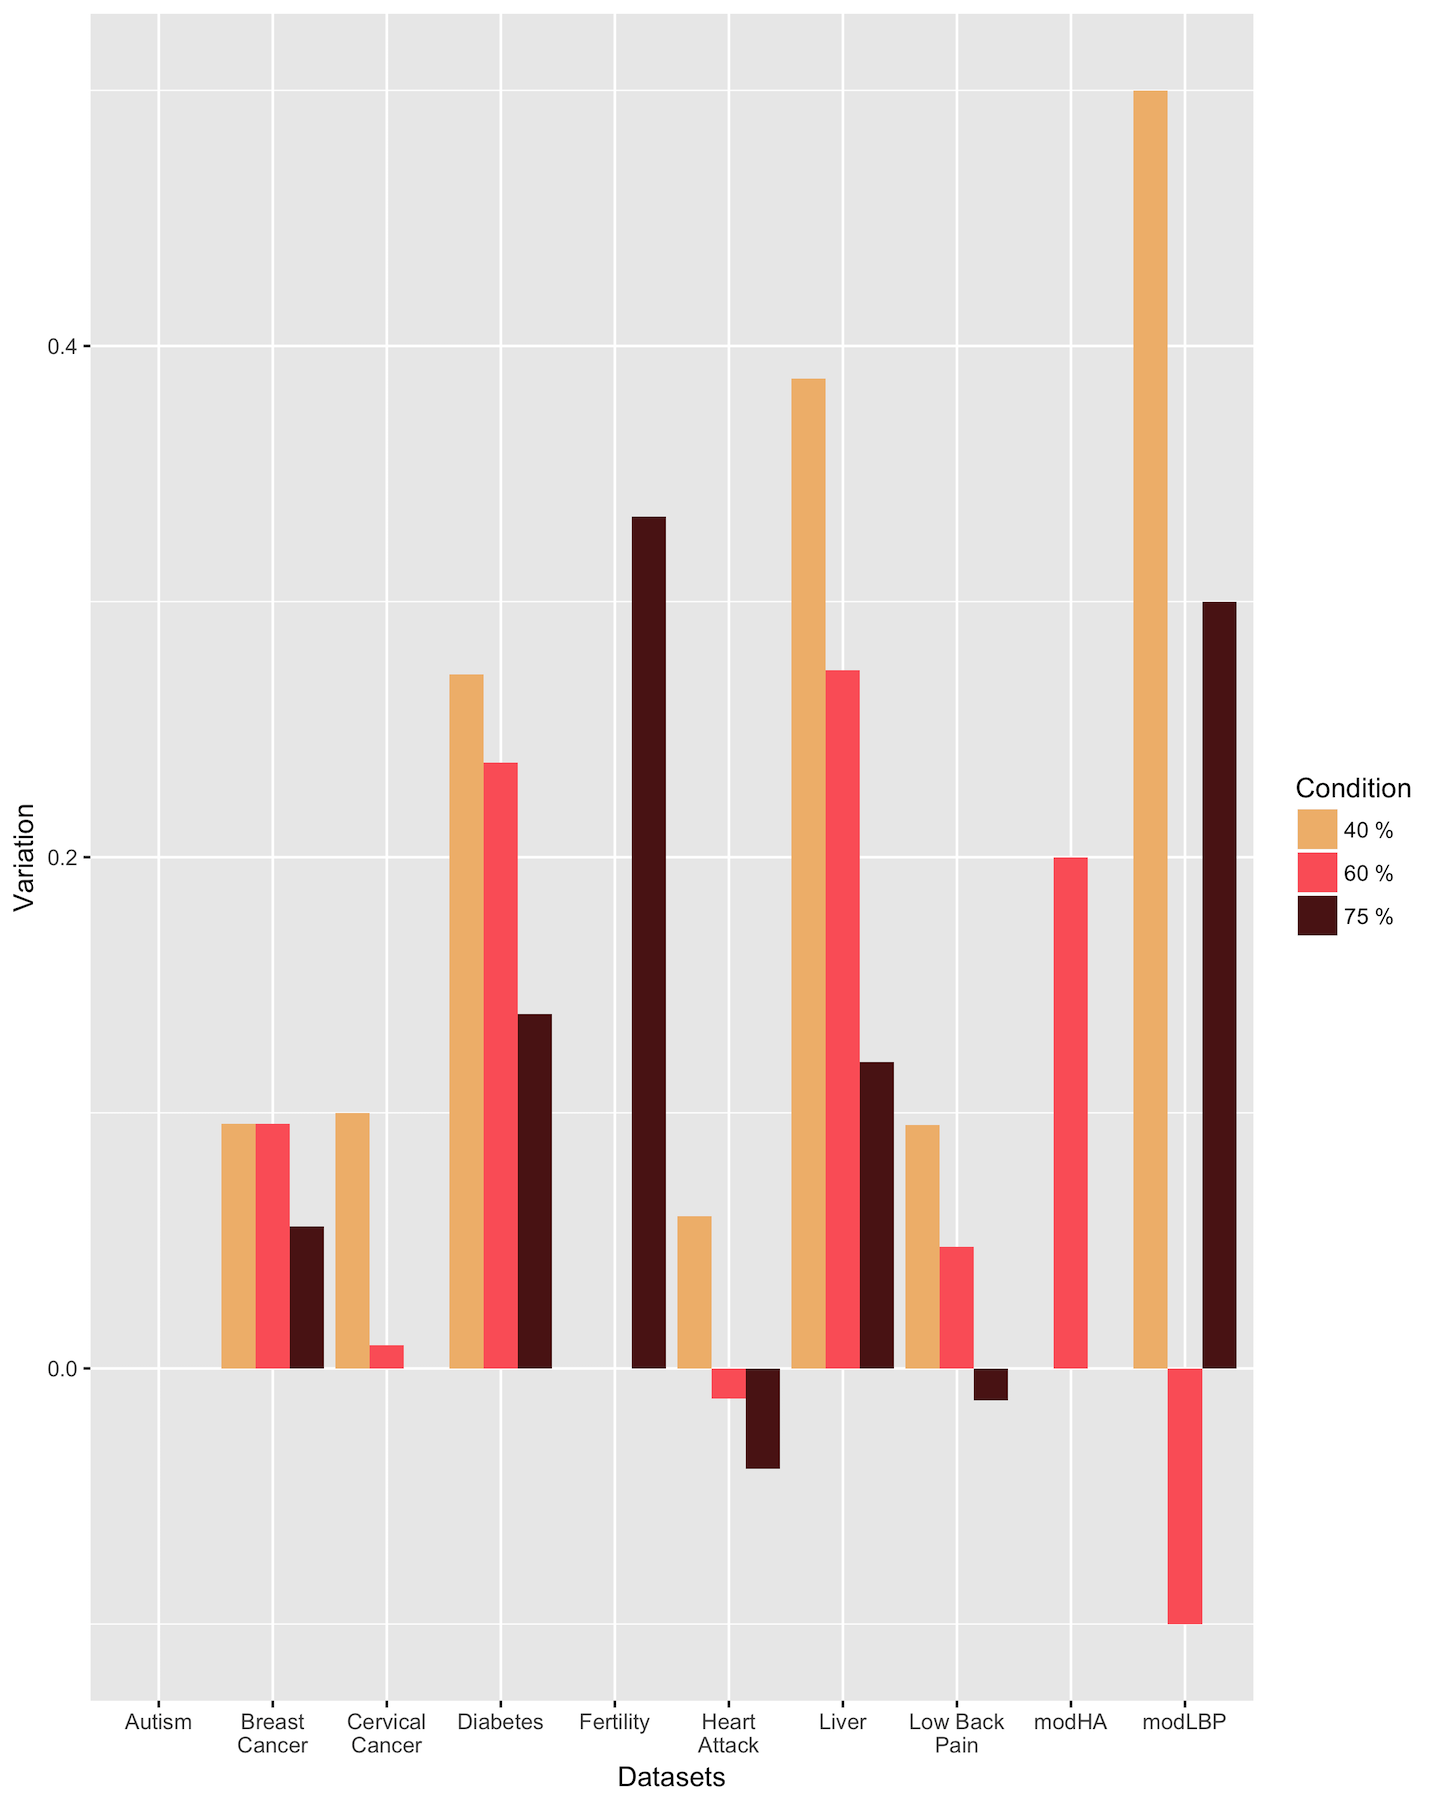
\includegraphics[width=0.9\textwidth]{ThesisTemplate/usingLatex/chapter5Images/SensiVariationUnderBySets.png}
    \caption{Variation of the sensitivity value for the three under-sampling conditions compared to the baseline established in Experiment 1 for all studied datasets.}
    \label{fig:my_label}
\end{figure}
Figure 5.2 shows the variations in sensitivity observed when   75\%, 60\% and 40\% of the majority class was retained. The overall effect is that sensitivity increases when under-sampling is applied; The trend is that the more of the majority class has been discarded, the more the sensitivity increases, the highest observed increase is 0.4.\newline



\begin{figure}[!htbp]
    \centering
    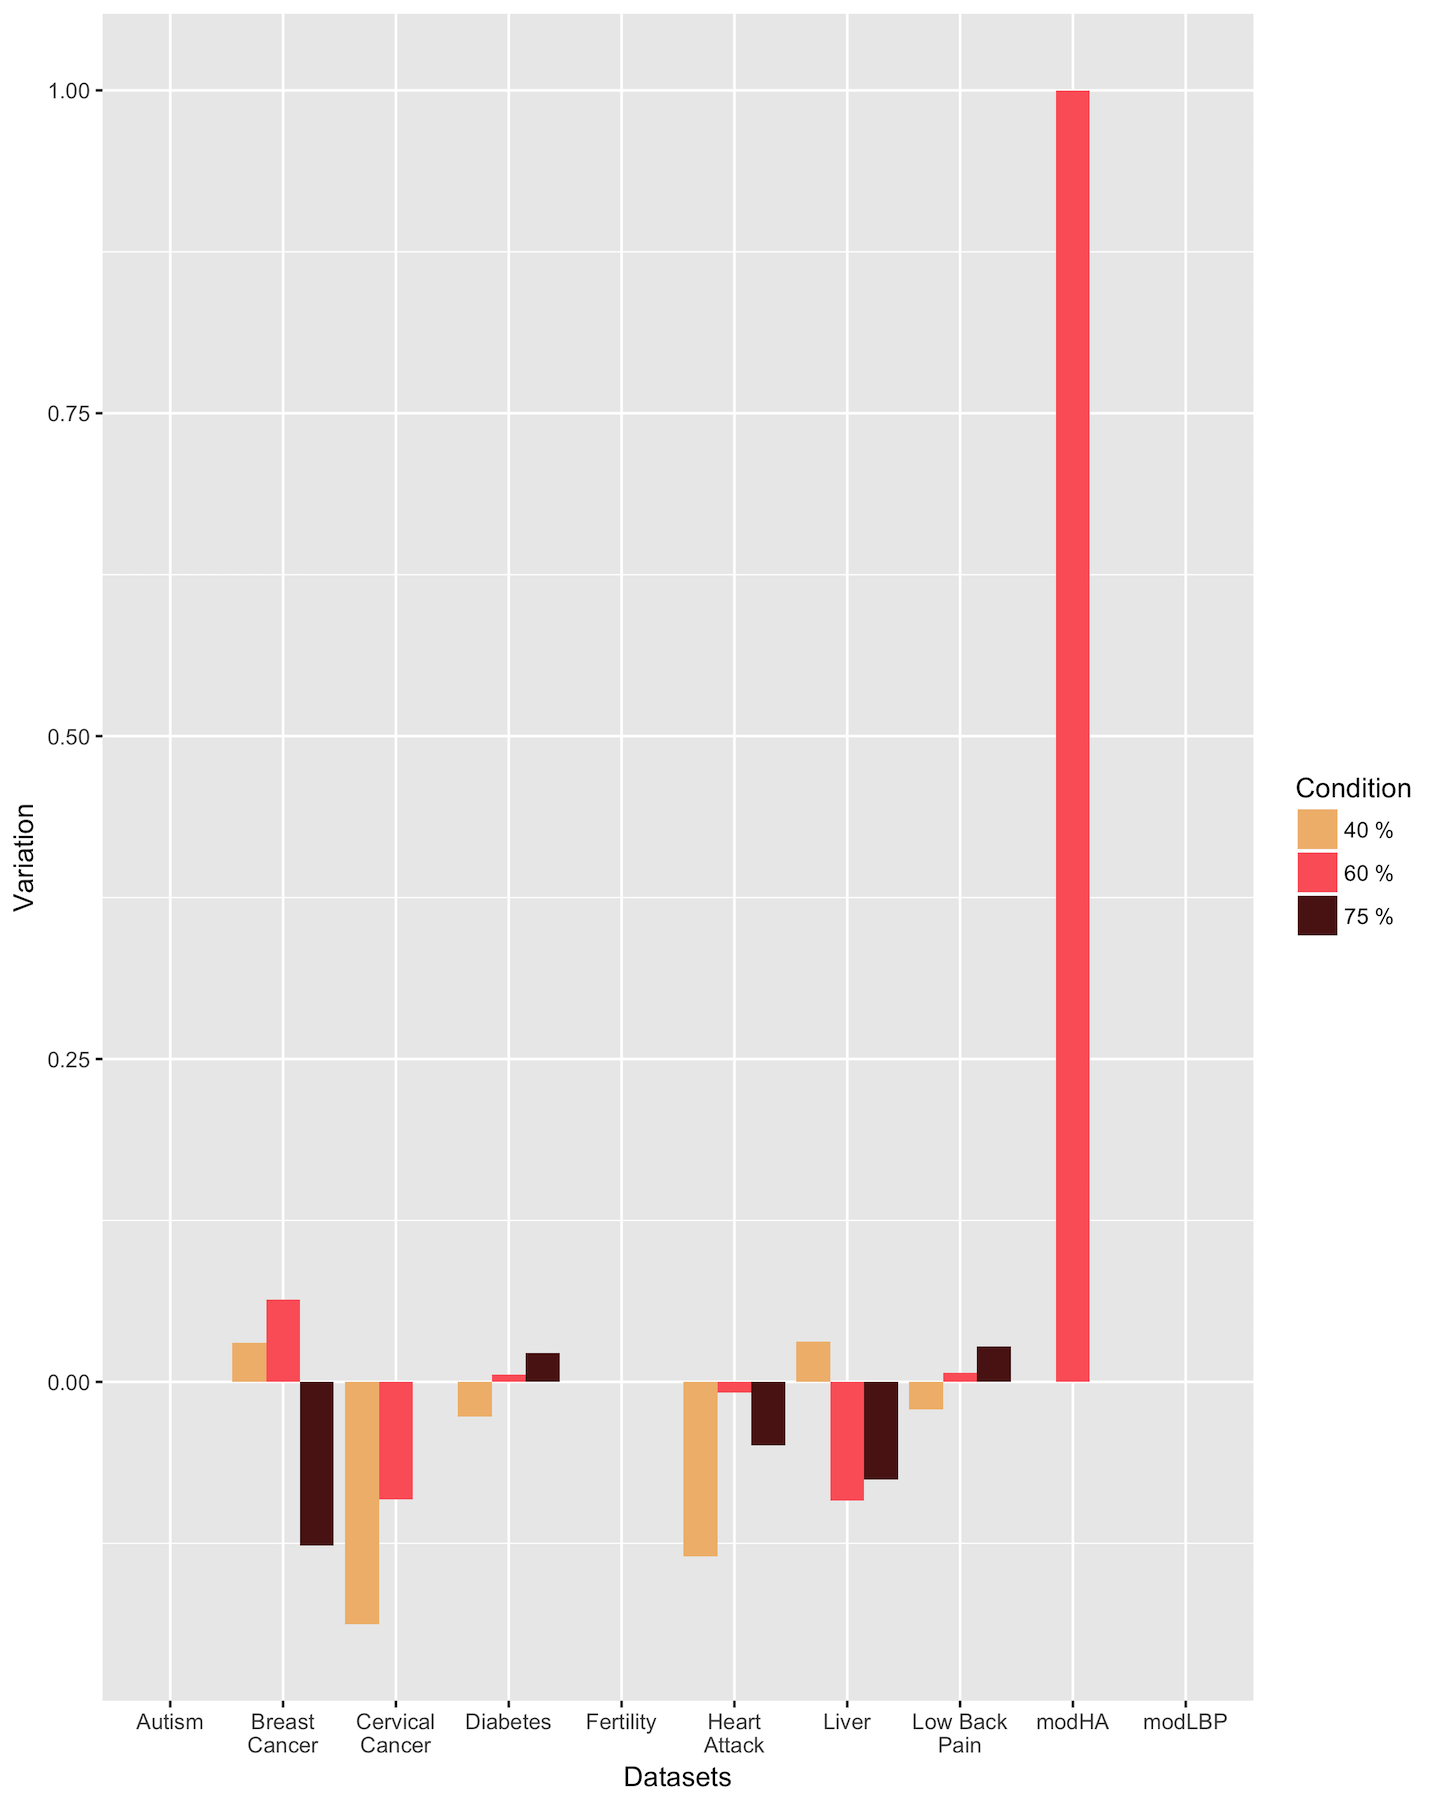
\includegraphics[width=0.9\textwidth]{ThesisTemplate/usingLatex/chapter5Images/PreciVariationUnderBySets.png}
    \caption{Variation of the precision value for the three under-sampling conditions compared to the baseline established in Experiment 1 for all studied datasets.}
    \label{fig:my_label}
\end{figure}

Figure 5.3 shows the variations in precision observed when 75\%, 60\% and 40\% of the majority class was retained. In general, precision is reduced by under-sampling, particularly if the proportion of the majority class to be discarded is large, though the effect remains light (maximum reduction is 0.19) In one case (modified Heart Attack dataset), the precision value is greatly increase when 60\% of the majority class is retained, though that effect is not consistent with what is observed on the other datasets.\newline

\begin{figure}[!htbp]
    \centering
    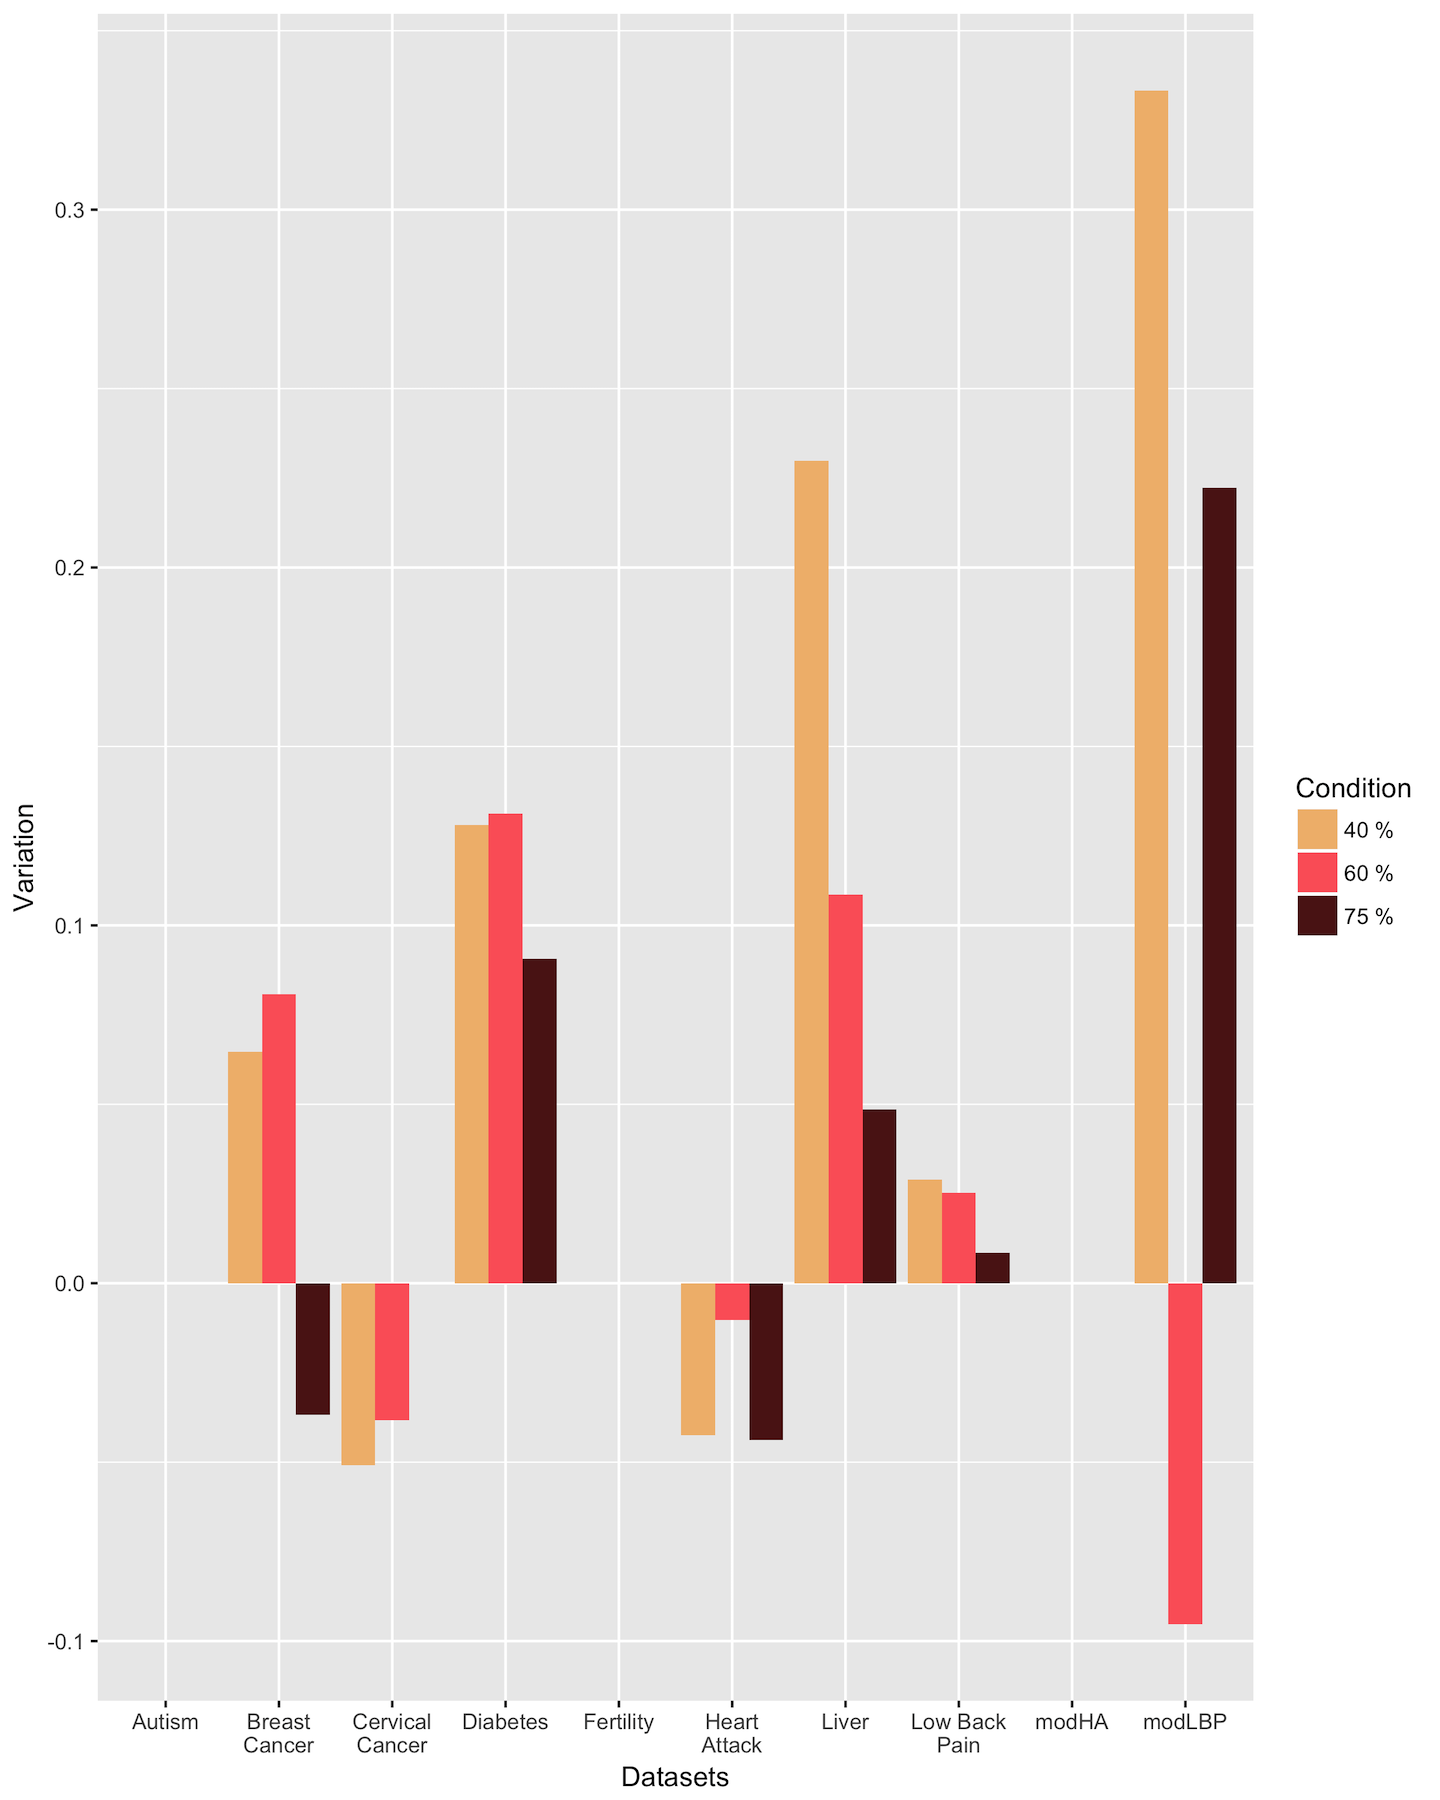
\includegraphics[width=0.9\textwidth]{ThesisTemplate/usingLatex/chapter5Images/F1VariationUnderBySets.png}
    \caption{Variation of the F1 score value for the three under-sampling conditions compared to the baseline established in Experiment 1 for all studied datasets.}
    \label{fig:my_label}
\end{figure}

Figure 5.4 shows the variations in F1 score observed when 75\%, 60\% and 40\% of the majority class was retained. In general the F1 score increases with the increased proportion of discarded majority class. The F1 score is partly dependent on both precision and sensitivity, but as previously discussed sensitivity tends to increase when the proportion of majority class discarded increases while precision decreases when the proportion of majority class discarded increases but to a lesser extent; thus the overall effect on the F1 score is that it increases as the proportion of majority class discarded increases.\newline

\subsection{Over-sampling the minority class (SMOTE)}
Over-sampling was carried out using the smote() function of R (see script Experiment3.R).

\section{Discussion}
\subsection{Under-sampling}
Statistical analysis was carried out on the values obtained from Experiments 1 and 2. An independent t-test was carried out using the software SSPS to evaluate the significance of the variations for each metrics between the baseline (no under-sampling) and each under-sampling condition.\newline
The output files from SSPS can be found in the github repository and in the appendix. Table 5.5. shows the 2-tail t-test sigma values obtained for each test. All tests were carried out with and without the values for the Autism dataset as these remained unchanged in all experiments and may have affected the results of the t-test.
None of the sigma values are inferior to 0.05, which means that the observed differences are not significant. It is however worth noting that the samples for each test is small as only 10 datasets were analysed and in some cases the precision or F1 score values were not available, further reducing the number of available cases to be considered. A more extensive analysis with a larger number of datasets could potentially yield statistically significant results.\newline

\begin{table}[!htbp]
\centering
\begin{tabular}{*9c}
  \hline
  \rowcolor{LightCyan}
Condition &\multicolumn{2}{c}{Accuracy} &\multicolumn{2}{c}{Sensitivity} &\multicolumn{2}{c}{Precision}&\multicolumn{2}{c}{F1.Score}\\
  \hline
           & [A] & [B] & [A] & [B] & [A] & [B] & [A] & [B] \\
Under 40  &0.608& 0.581& 0.395 & 0.375 & 0.820 & 0.815 & 0.297 & 0.255 \\ 
  Under 60 &0.353& 0.318& 0.649 & 0.628 & 0.941 & 0.925 & 0.789 & 0.800 \\ 
  Under 75 &0.797&0.783 & 0.570 & 0.544 & 0.476 & 0.476 & 0.999 & 0.967 \\ 
   \hline
\end{tabular}
\caption{2-tail t-test sigma values for independent t-test carried out on the results obtained for accuracy, sensitivity, precision and F1 score for each of the datasets. [A] Values obtained while keeping the results for the Autism dataset, [B] values obtained while removing the results obtained for the Autism dataset as they were unchanged in any of the conditions.}
\end{table}








 

\section{Conclusions}

The main conclusions for this chapter.


